\documentclass[a4paper]{article}
\usepackage{a4wide}
% \usepackage{graphicx}
% \usepackage{amssymb,amsmath}
% \usepackage{booktabs}
\usepackage[english]{babel}
% \usepackage{multirow}
\usepackage{graphicx}% Include figure files
% \usepackage{color}
\emergencystretch=35pt
\usepackage[pdftex,unicode,colorlinks, citecolor=blue,%
filecolor=black, linkcolor=blue, urlcolor=black]{hyperref}
\usepackage[figure,table]{hypcap}


\begin{document}
\begin{center}
  Response Letter
\end{center}
Dear Editors,
\\
\\
I am writing to respond to the reviewers' critical comments on our
manuscript entitled, ``Superabsorption of light by nanoparticles''
NR-COM-08-2015-005468, which we aim for publication in Nanoscale.

As a group of authors interested in high quality input we know that
unbiased and professional review is an important part of a publication
process.  This way we would like to stress you attantion to the second
comment of the first reviewer. He had listed a number of publications,
however, it is hard to belive that this list is unbiased after looking
to the authors names; several authors from Jiangxi Normal University are
listed in all of this publications (it looks like some names have two
spelling options with and without the dash).  We provide our findings here:
\begin{enumerate}
\item ACS Applied Materials & Interfaces, 7, 4962-4968 (2015)\\
  Zhengqi Liu, Xiaoshan Liu,  Shan Huang,  Pingping Pan,  Jing Chen,
  Guiqiang Liu, and Gang Gu\\
  DOI: 10.1021/acsami.5b00056
\item Materials Letters 158, 262-265 (2015)\\
  Zhengqi Liu , Guiqiang Liu, Xiaoshan Liu, Shan Huang, Yan Wang,
  Pingping Pan, Mulin Liu\\
  http://dx.doi.org/10.1016/j.matlet.2015.06.029
\item Applied Physics Letters, 104, 081116 (2014)\\
  Zheng-qi Liu, Hui-bai Shao,  Gui-qiang Liu, Xiao-shan Liu, Hai-qing Zhou, Ying Hu,
  Xiang-nan Zhang, Zheng-jie Cai, and Gang Gu\\
  http://dx.doi.org/10.1063/1.4867028
\item Nanotechnology, 24, 155203 (2013)\\
  Zheng-qi Liu, Gui-qiang Liu, Hai-qing Zhou, Xiao-shan Liu,
  Kuan Huang, Yuan-hao Chen, and Guo-lan Fu\\
  doi:10.1088/0957-4484/24/15/155203
\end{enumerate}

We would like to thank the editor and two anonymous reviewers for their
constructive comments, which helped us to improve the
manuscript. Below, we address all comments point-by-point, discussing
the subsequent modifications.

\vspace{10pt}

\newpage
\textbf{Reviewer \#1 comments}

\begin{tabular}[!H]{l|p{0.9\textwidth}}
\quad & 1. The authors claimed “Combined effect of these resonances is presented to produce the flat and relative broadband electric resonance response.” Nevertheless, the broadened absorption band is not very broad. Is there any further way to predict a broadband light absorption. For instance, a broadband absorption in the whole visible spectral range. Maybe, a possible way of using the dispersed size scale nanoparticles should be added for improving the study. 
\end{tabular}\\

This comment touches two aspects of broadband performance, namely,
properties of a stanalone particle and in interaction with other
particles.  The first case, as it was correctly mentioned with the
reviewer, has some limiations.  We can design a band, which will be
broader of a typical band for a given multipole, however, width is
not extremly large.  To illustrate this we have run an optimization
with a goal to provide a prediefined separation between multipole
resonanses (Fig.~\ref{fig:broadband}).
\begin{figure}
  \begin{minipage}[h]{0.49\textwidth}    \begin{flushleft}     a)    \end{flushleft}
  \end{minipage}
  \begin{minipage}[h]{0.49\textwidth}    \begin{flushleft}     b)    \end{flushleft}
  \end{minipage}
  \begin{minipage}[h]{0.49\textwidth} 
   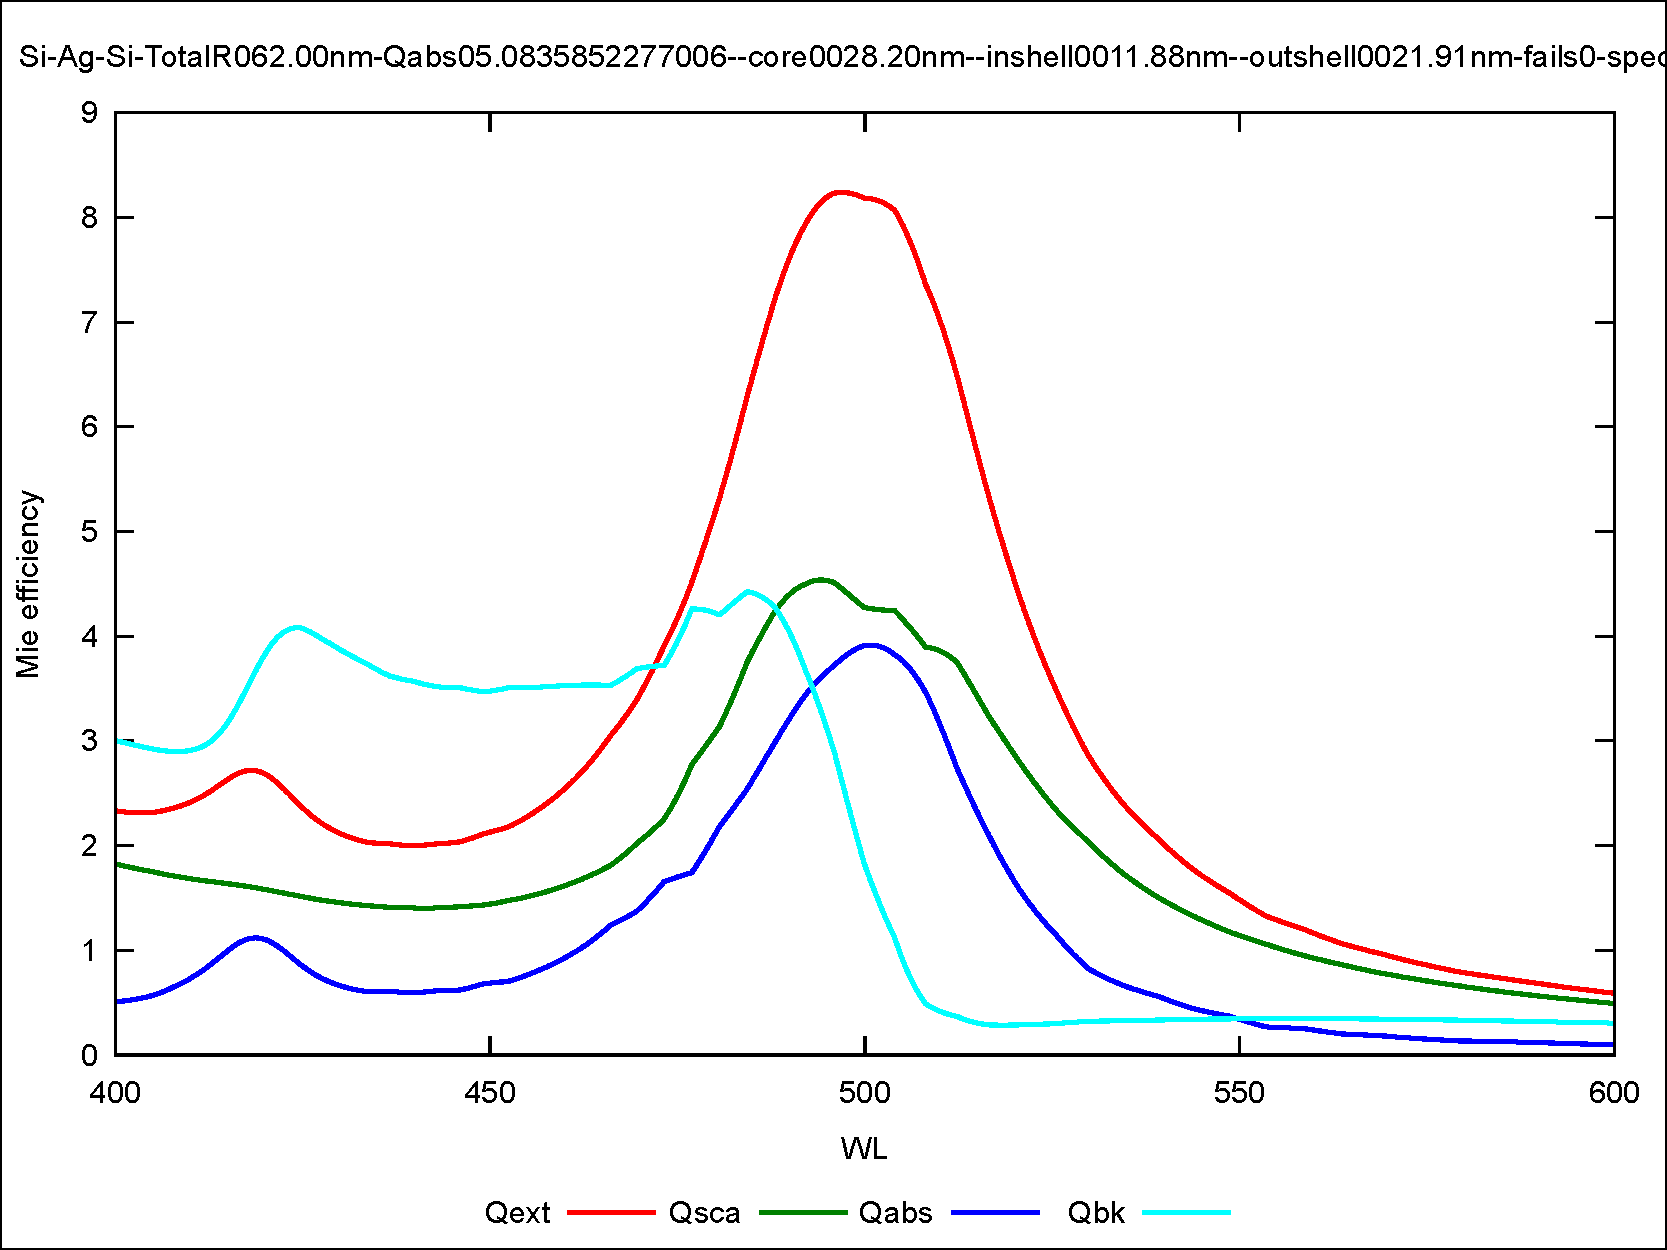
\includegraphics[width=0.95\textwidth]{band20-em}
  \end{minipage}
  \begin{minipage}[h]{0.49\textwidth} 
   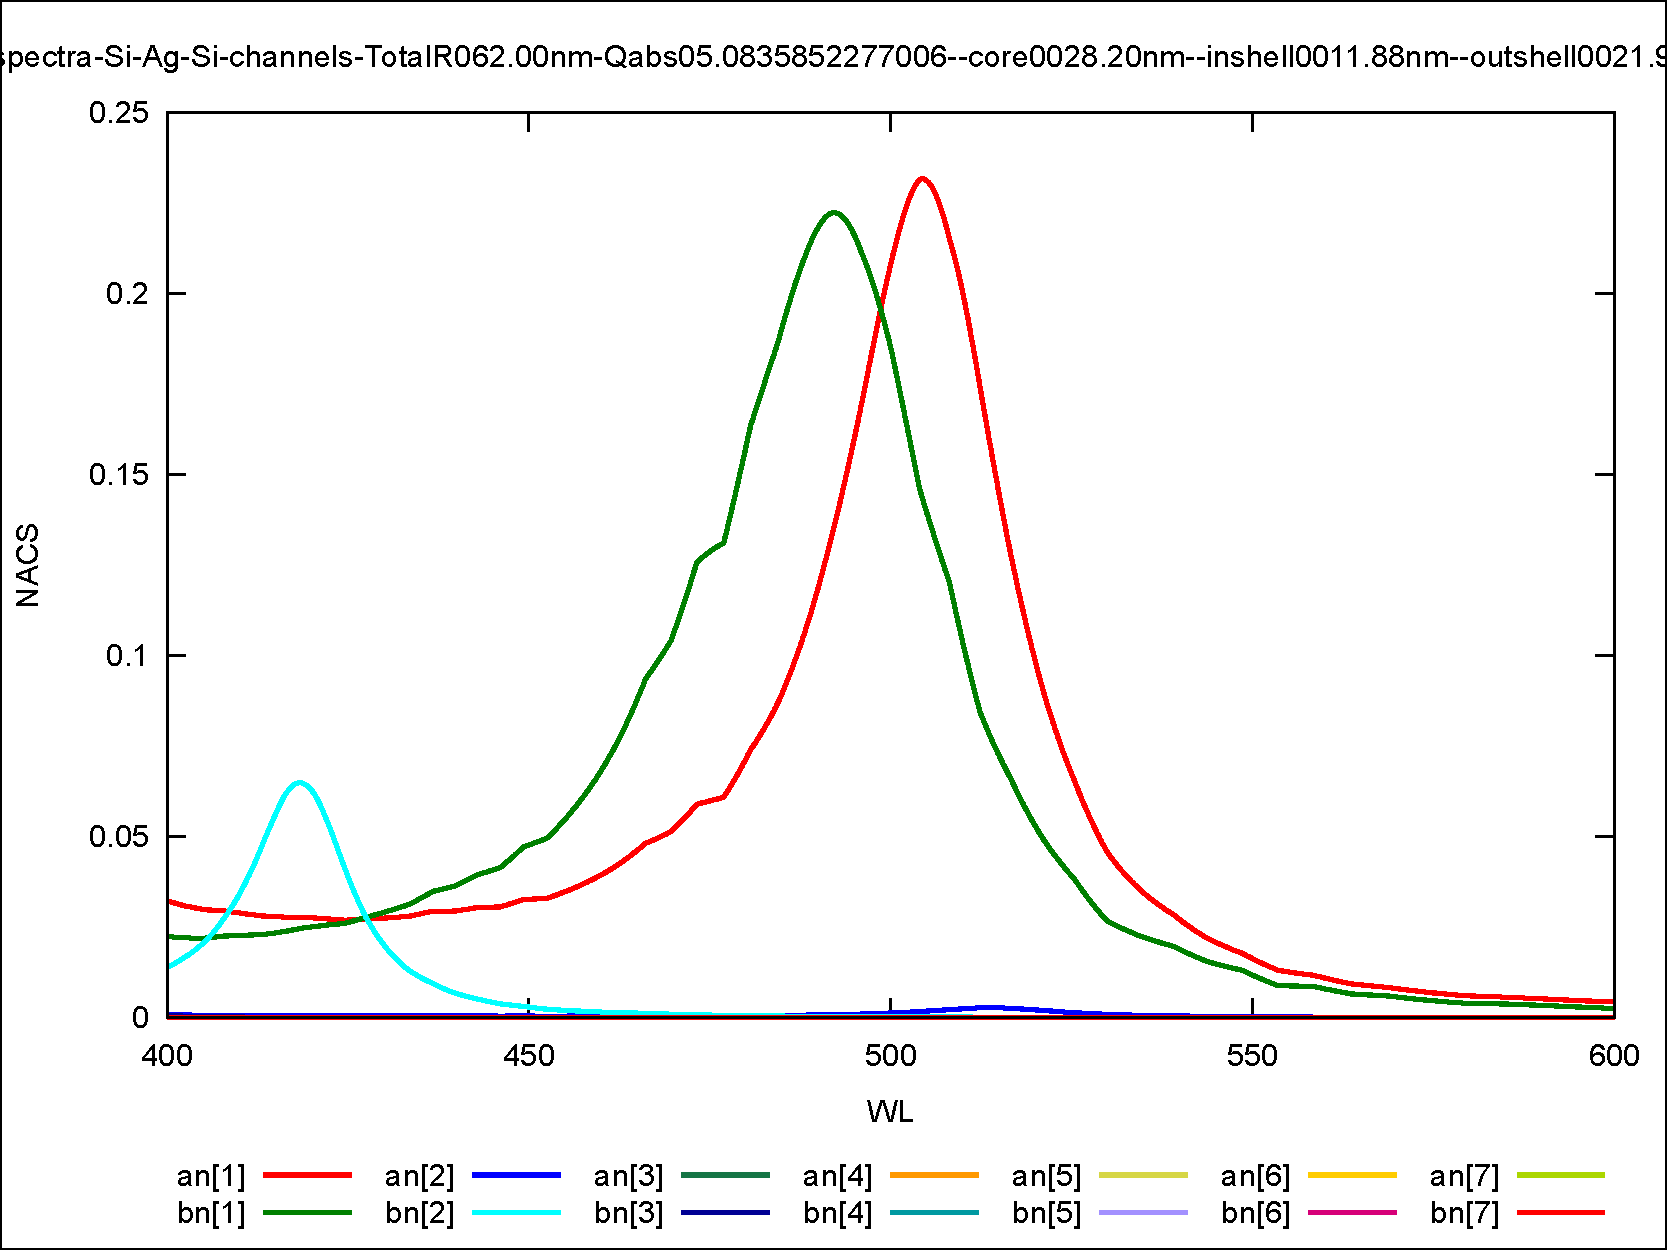
\includegraphics[width=0.95\textwidth]{band20-em-ch}
  \end{minipage}
  \begin{minipage}[h]{0.49\textwidth}    \begin{flushleft}     c)    \end{flushleft}
  \end{minipage}
  \begin{minipage}[h]{0.49\textwidth}    \begin{flushleft}     d)    \end{flushleft}
  \end{minipage}
  \begin{minipage}[h]{0.49\textwidth} 
   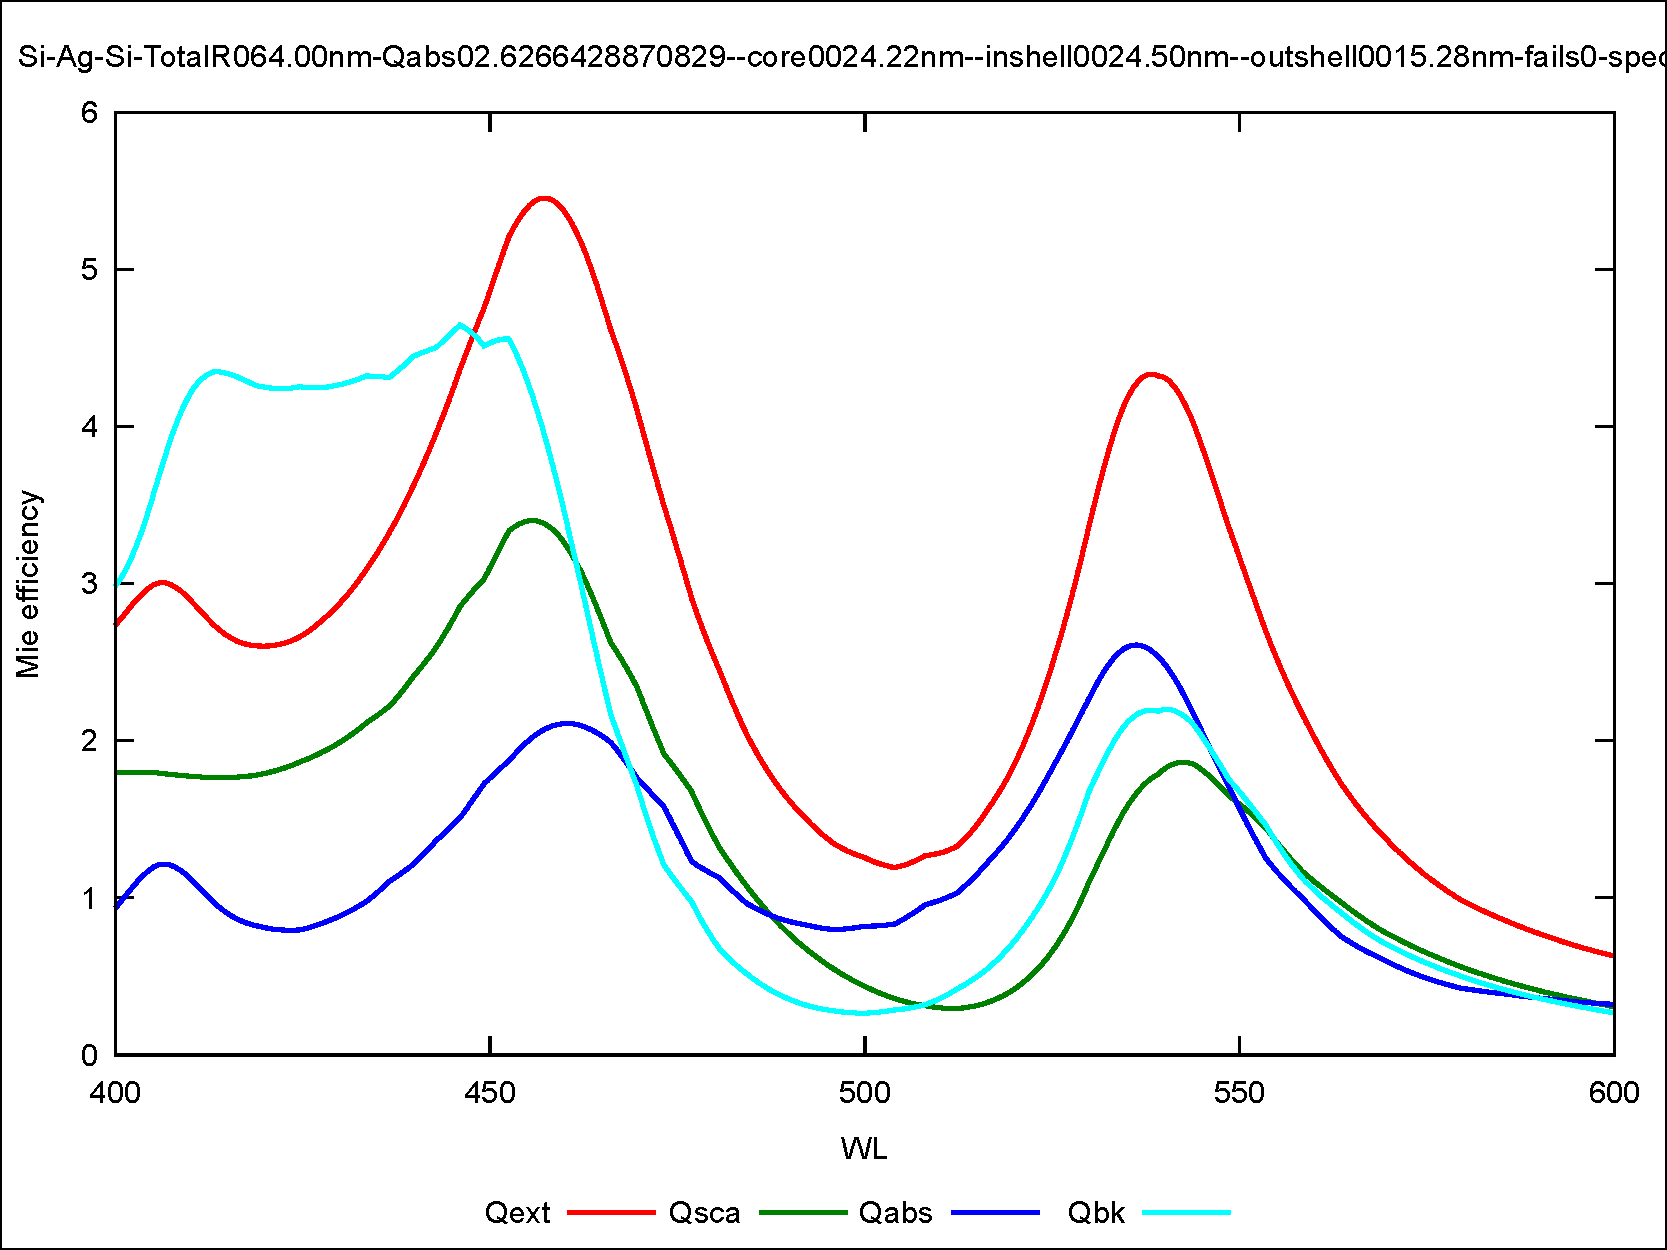
\includegraphics[width=0.95\textwidth]{band80-em}
  \end{minipage}
  \begin{minipage}[h]{0.49\textwidth} 
    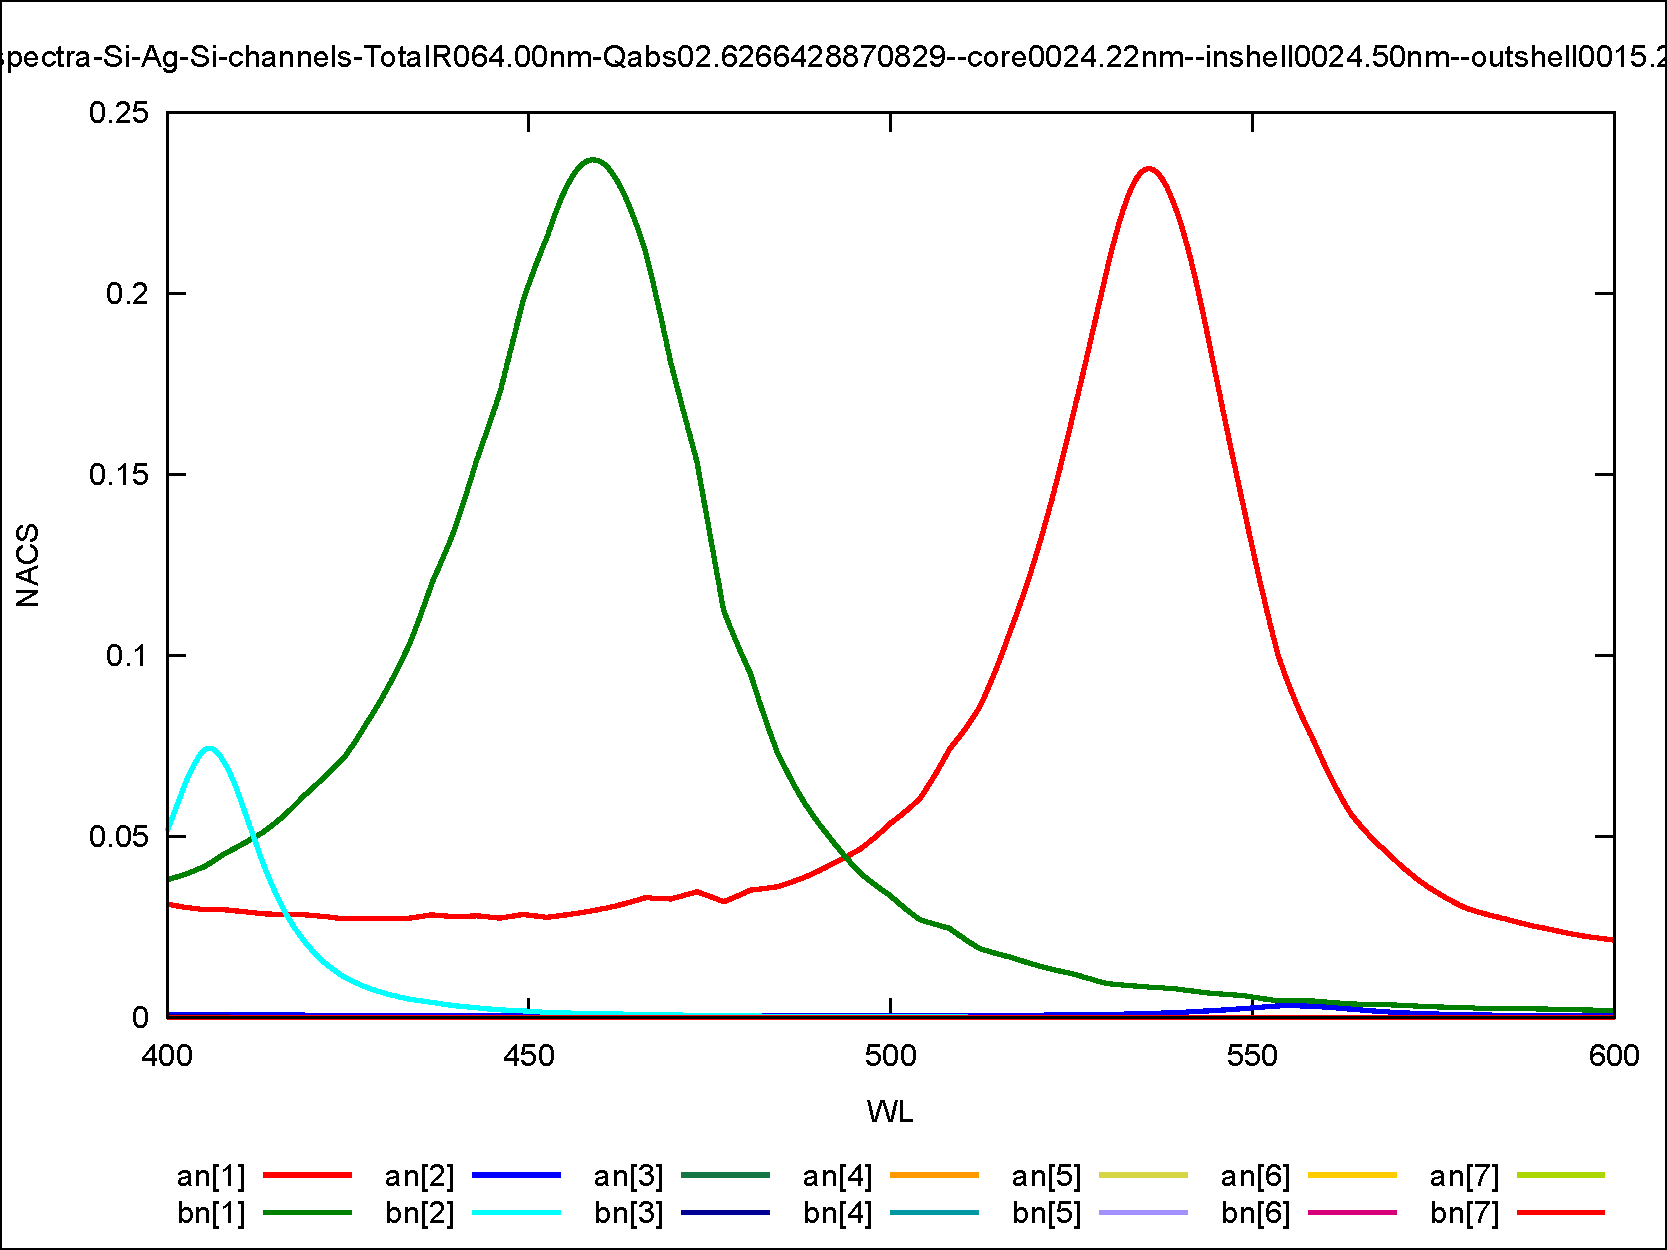
\includegraphics[width=0.95\textwidth]{band80-em-ch}
  \end{minipage}  
  \begin{minipage}[h]{0.49\textwidth}    \begin{flushleft}     e)    \end{flushleft}
  \end{minipage}
  \begin{minipage}[h]{0.49\textwidth}    \begin{flushleft}     f)    \end{flushleft}
  \end{minipage}
  \begin{minipage}[h]{0.49\textwidth} 
   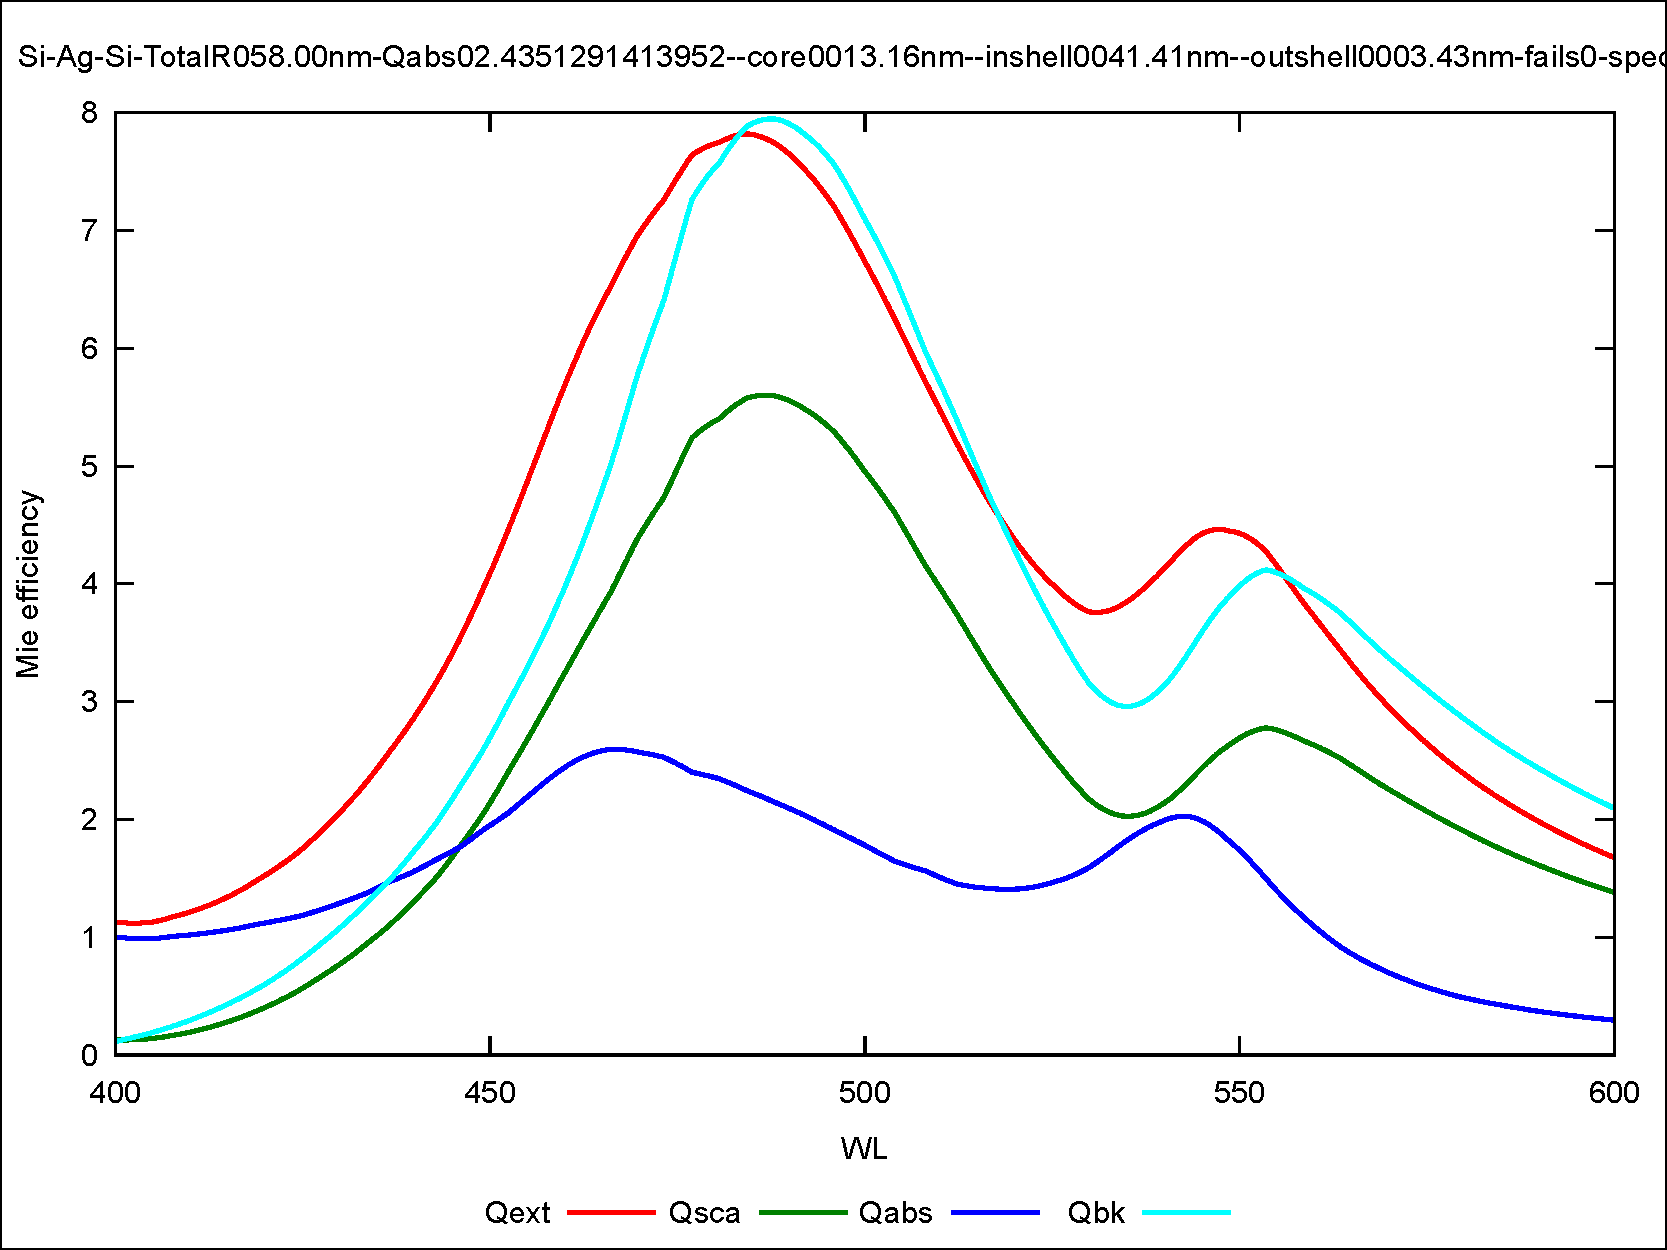
\includegraphics[width=0.95\textwidth]{band80-e}
  \end{minipage}
  \begin{minipage}[h]{0.49\textwidth} 
    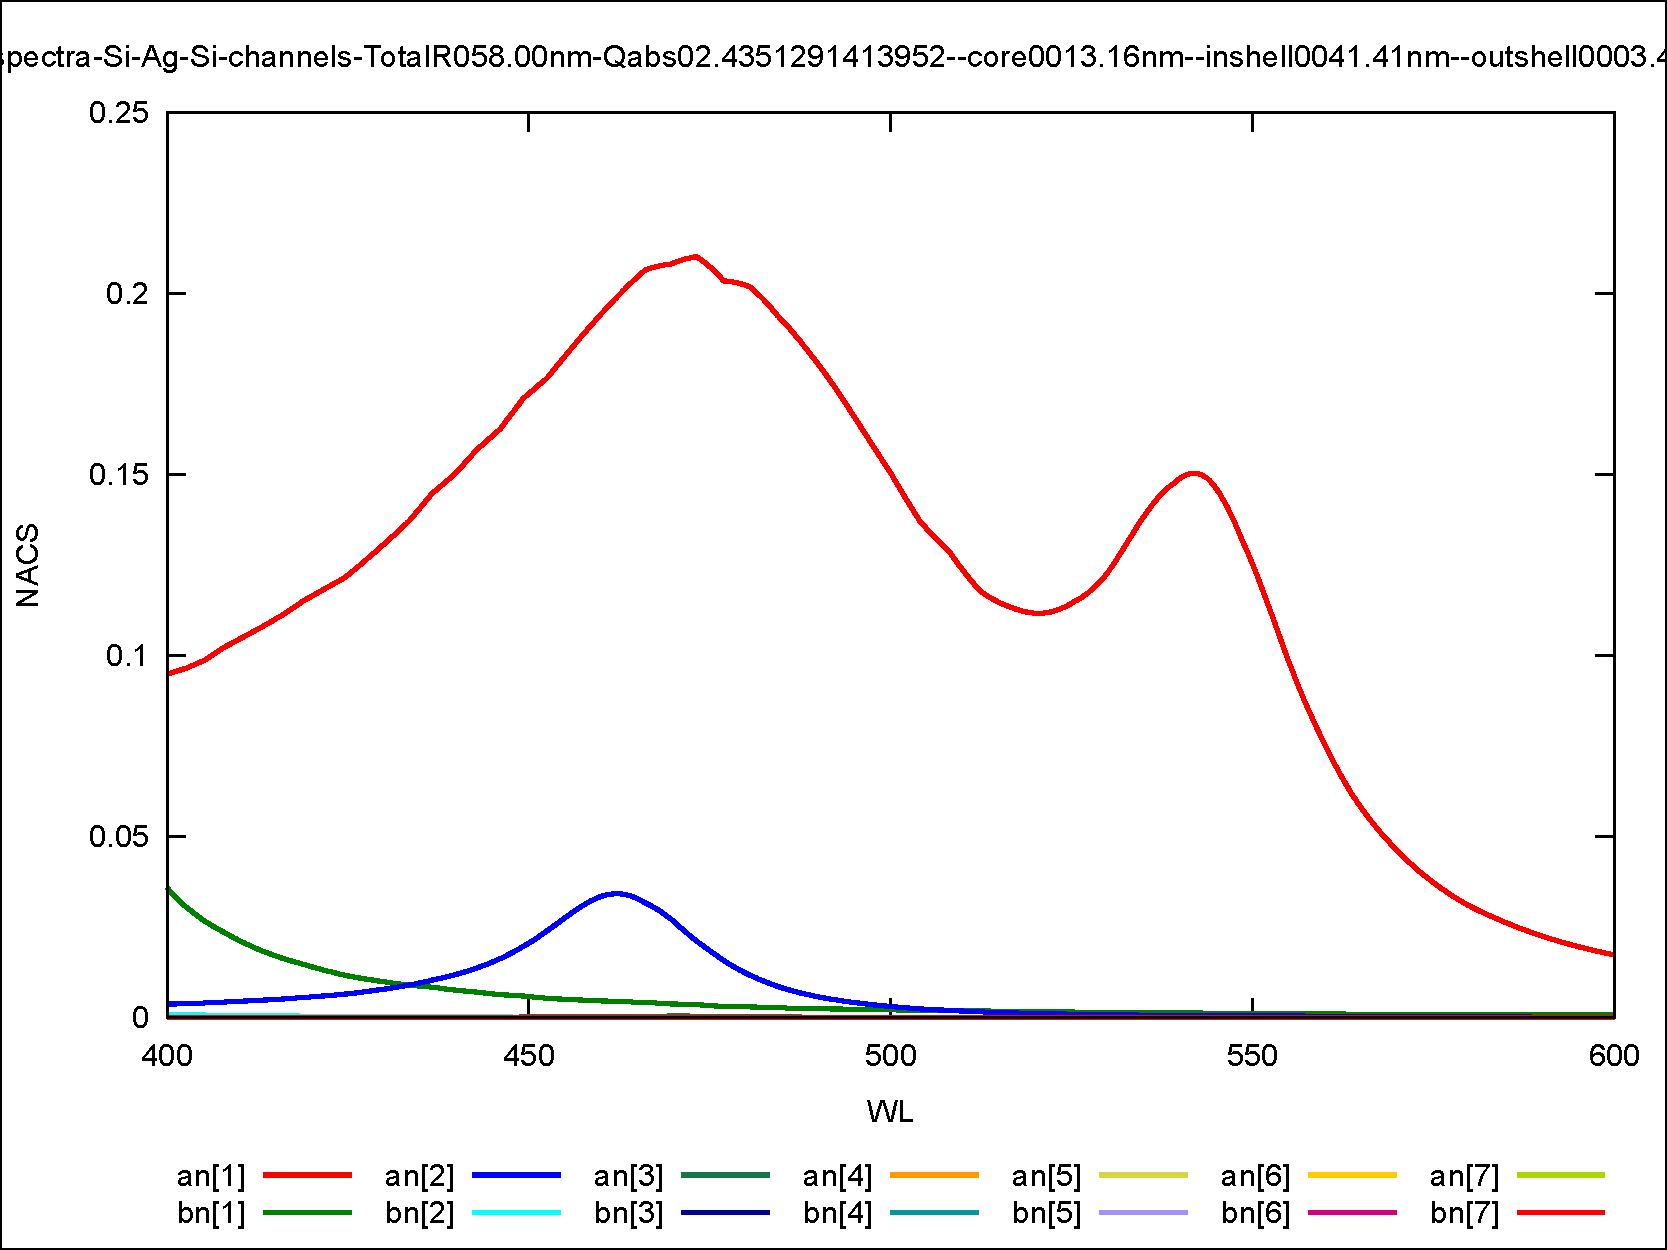
\includegraphics[width=0.95\textwidth]{band80-e-ch}
  \end{minipage}  
   \caption{Single particle desings for separation between dipole
     resonances of 20 nm (a-b) and 80 nm (c-f). Left column with
     figures (a,c,e) contains spectra of Mie efficiency for extinction
     (Qext), scattering (Qsca), absorption (Qabs, blue curve) and
     backscattering (Qbk). Right column (b,d,f) presents contibution
     of multipoles to the spectra (red and green stands for electric
     and magnetic dipoles, blue and cyan corresponds to quadrupole
     electric and magnetic modes, respectively). It is interesting to
     note that for 80 nm separation optimizer was able to find a
     desing with two resonances of a dipole mode (f). We suppose that
     the latter most likely has the same nature as the response
     presented in Fig. 3(c,d) of the manuscript: there are several
     resonances of an electric dipole response binded to different
     layers of the particle.\label{fig:broadband}}%
\end{figure}
Our observation is the following: while the separation is small enough
compared to a multiple resonance width the optimizer was successful to
find desings with electric and magnetic dipole. If the separation is
large the absorption band splits into two. For large separation is is
also possible to obtain two resonanses of the electric dipole
response, located at predefined position
(Fig. \ref{fig:broadband}(e,f)).  Still there are not so many
possibilities here to design a good broadband. To control the
bandwidth at a given spectral position we need to involeve relatively
large particles. This leads to appereance of resonances (and
absorbtion) out of the designed band which are hard to control or
suppress in disscussed triple-layer structure.

To answer the second part of the comment, related to possiblity of
usage of the pariticle array with dispered sizes, we designed two
particles with best absorption effeciency at 475~nm and 525~nm (outer
radius 34 and 38~nm) and
simulatied them both with FDTD method using Lumerical FDTD Solutions.
Sketch of the simulated system and final results are in
Fig.~\ref{fig:fdtd}. To verify our FDTD we fist simulated absorption
of standalone spheres, the obtained postions and amplitudes of
resonances to corresponde well with Mie caclulations.
\begin{figure}
  \begin{minipage}[h]{0.49\textwidth}    \begin{flushleft}     a)    \end{flushleft}
  \end{minipage}
  \begin{minipage}[h]{0.49\textwidth}    \begin{flushleft}     b)    \end{flushleft}
  \end{minipage}
  \begin{minipage}[h]{0.49\textwidth} 
   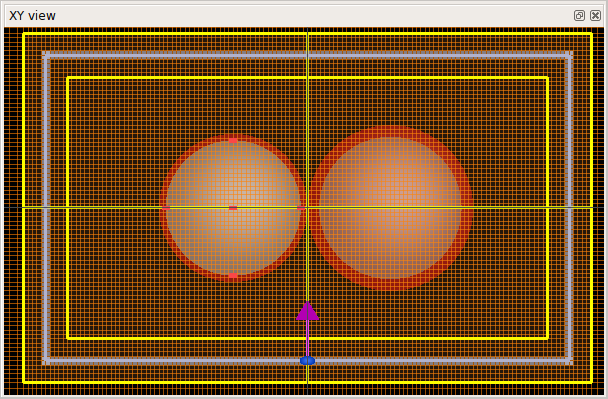
\includegraphics[width=0.95\textwidth]{FDTD-mode-d00}
  \end{minipage}
  \begin{minipage}[h]{0.49\textwidth} 
   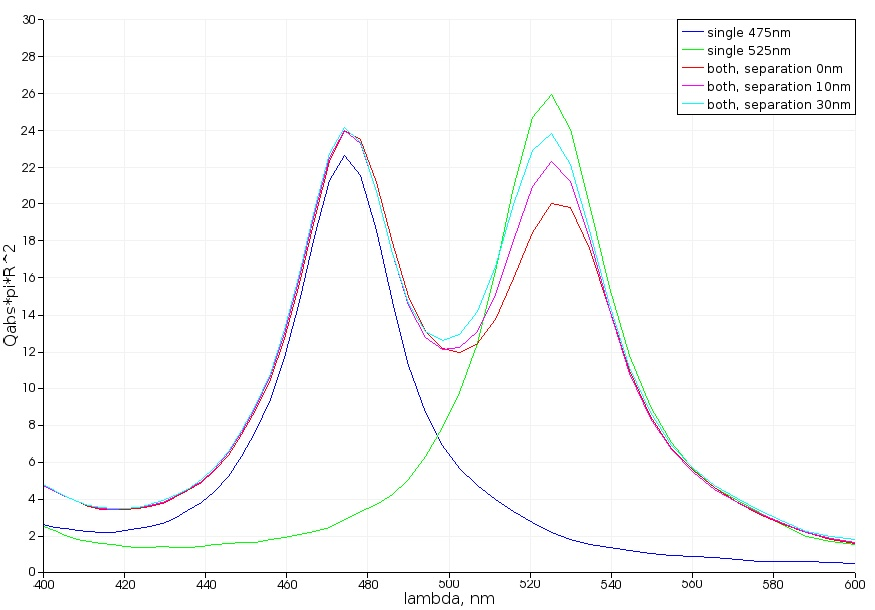
\includegraphics[width=0.95\textwidth]{fdtd-spectra}
  \end{minipage}
  \begin{minipage}[h]{0.49\textwidth}    \begin{flushleft}     c)    \end{flushleft}
  \end{minipage}
  \begin{minipage}[h]{0.49\textwidth}    \begin{flushleft}     d)   \end{flushleft}
  \end{minipage}
  \begin{minipage}[h]{0.49\textwidth} 
    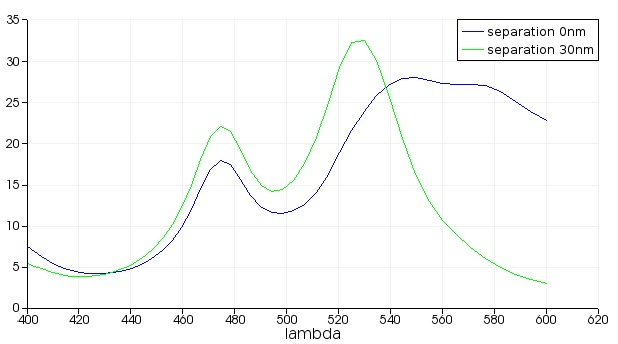
\includegraphics[width=0.95\textwidth]{fdtd-spectra-Ek}
  \end{minipage}
  \begin{minipage}[h]{0.49\textwidth} 
    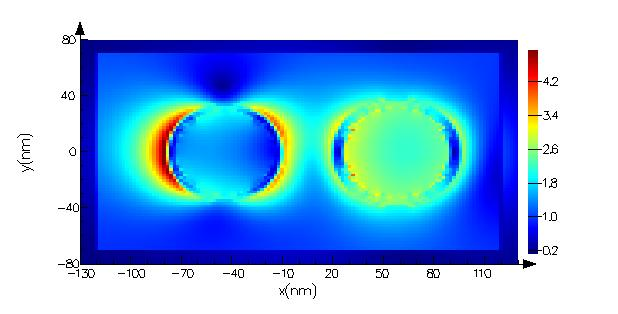
\includegraphics[width=0.95\textwidth]{fdtd-field}
  \end{minipage}
    \caption{(a) Fullwave simulation prepared in Lumerical FDTD. (b)
     Absorption spectra of stand-alone spheres and in dimer
     configuration with separation between spheres of 0, 10, and
     30~nm, particles are in H-k plane (c) Separation 0 and 30~nm for
     particles in E-k plane (d) Field distribution at 500nm of
     incedent wavelength for particles in E-k plane with separation of
     30~nm.\label{fig:fdtd}}%
\end{figure}
Next step was to find out the possible interactions between two
spheres, so we run a simulation in dimer configuration with zero
separation between spheres and with 10 and 30~nm separation.  The
resulting spectra has a strong contribution from standalone
resonances, while coupling effects seems to be minor.  This can be
easily explained from field distribution in Fig.~4(c) of the
manuscript. Positioning spheres in H-k plane we are exploting the
feature of field being highly localized inside the the sphere.  For
sure arranging spheres in other plane, increasing the number of
spheres can change the amount of coupling between the spheres. As an
example we tested arragement of sphers in E-k plane
Fig.~\ref{fig:fdtd}(c); for zero separation the intraction between
spheres is strong, however, due to near-field nature of this coupling
it rapidly decays with the separation width Fig.~\ref{fig:fdtd}(d),
for separation of 30~nm responses of individual particles dominate in
overall spectra for both planes of polarization. This way we show that
in principle it is possible to construct an absoption band of an array
of dispersed particles simply optimizing the properties of every
single sphere carefully tuning the distance between particles (which
still is much smaller than the wavelength).

We changed the manuscript from ``As a result, one can design
spectrally-selective absorbers or broadband absorbers with almost
arbitrary prescribed properties.'' to ``As a result, one can design
absorbers with broadened spectra or spectrally-selective absorbers
with almost arbitrary prescribed properties.  Due to strong
localization of electric dipole field (espatially in H-k plane) it is
also possible to desing dispersed size arrays particles by defining
their individual properties for composite absorption spectra; we
obtained rather small coupling between particles during additional
simulation using FDTD method.''

% band80-e
% Si-Ag-Si-TotalR058.00nm-Qabs02.4351291413952--core0013.16nm--inshell0041.41nm--outshell0003.43nm-fails0-spectra
% band80-em
% Si-Ag-Si-TotalR064.00nm-Qabs02.6266428870829--core0024.22nm--inshell0024.50nm--outshell0015.28nm-fails0-spectra
% band20-e
% Si-Ag-Si-TotalR058.00nm-Qabs03.9125128013731--core0010.44nm--inshell0042.75nm--outshell0004.81nm-fails0-spectra
% band20-em
% Si-Ag-Si-TotalR062.00nm-Qabs05.0835852277006--core0028.20nm--inshell0011.88nm--outshell0021.91nm-fails0-spectra

%% 400-700 3-layer
%% 4-layer?

%% В статье этого графика нет, есть обсуждение, готовим новую статью.
%% In order to reply to this comment we run an optimization ...




\begin{tabular}[!H]{l|p{0.9\textwidth}}
  \quad & 2. To achieve super-absorption behavior, it is interesting
  to know what will happen when the multilayered nanoparticles are
  closely packed as the plasmonic crystal. As reported in the previous
  papers [ACS Applied Materials \& Interfaces, 7, 4962−4968 (2015);
  Materials Letters 158, 262–265 (2015); Applied Physics Letters, 104,
  081116 (2014); Nanotechnology, 24, 155203 (2013)], the packed
  plasmonic crystals have been demonstrated to show broadband light
  coupling and confinement. Thereby, it would be interesting to show
  improved broadband light absorption based on the plasmonic crystal
  of this proposed multilayered nanoparticles. 
\end{tabular}

% Lumerical - periodic boundary - попробовать несколько частиц
We would like to thank the reviewer for provided citations, some of
them turned to be really interesting. In order to reply this comment
first of all we checked all the citations provided.

ACS Applied Materials \& Interfaces, 7, 4962-4968 (2015) titled
``Automatically Acquired Broadband Plasmonic-Metamaterial Black
Absorber during the Metallic Film-Formation'' uses metal film
formation process to achive very wideband performance. However, the
absorption in this case is highly dependable on the thickness of the
underlaying silica layer.  This way we can argue against the conlusion
of the paper ``These results also confirm that an ultrathin
meta-surface layer (less than 10 nm) structure can produce nearly
ideal broadband light absorption'' - to achieve experimentally
observed performance the whole system (including silica layer and gold
under-layer) is needed. A more detailed simulation can give some
answers, however, we expect that most of the absorbtion happends in
the gold under-layer, while the metasurface and silica layer serves to
be kind of an impedance matcher.  This proposal is confirmed with the
experemental results in Fig. 5 of the paper, for 100~nm silica layer
the absorption is low.  At the same time the wideband performance can
be related to the fractal-type surface, as it is shown in Fig.~2(f)
Moreover, it should be relativly easy to estimate the thermal
behaviour of such a metasurface, as soon as isolated particles on the
top of the silica have no heat transfer with electrons to the
substrate.  If we suppose that most of the light is absorbed in top
layer this should lead to overheating of the metasurface due to
extreamly low geometrical volume. For this case in steady state we
should expect a large temperature gradient as soon as gold thermal
condutivity 310 $W/(m\cdot K)}$ is about 200 fold larger than silica
  $1.4 W/(m\cdot K)}$. Measuring temperature via infrared
    radiation from both sides of the sample can provide hints to
    distinguish the absortption origin.

Anyway, albiet of the exciting experimental results obtained in the
paper they exploit phsycal effect that differs a lot from the one
proposed in our manuscript; our particles were desinged to absorb the
incident power by themselfs, and they work perfectly in a stand-alone
mode.  This can be extremly conviniet, for example, for nanophotonics
application, when the available volume to place an absorber can be
very limited. Same overheating question can also appear here, limiting the
operational power range.



Applied Physics Letters, 104, 081116 (2014) titled ``$\lambda^3$/20000
plasmonic nanocavities with multispectral ultra-narrowband absorption
for high-quality sensing'' is cleary not related to ``broadband light
coupling and confinement'' and was
probably listed by an accident.

Nanotechnology, 24, 155203 (2013) titled ``Near-unity transparency of
a continuous metal film via cooperative effects of double plasmonic
arrays'' describes light interaction with a gold film, which has an
array of gold spheres positioned on top, bottom, or both sides of the
film.  Provided simulations show a strong field enhancement between
the spheres. Absorption related part of the paper references [18-21],
where [20] is Le F, Brandl D W, Urzhumov Y A, Wang H, Kundu J, Halas N
J, Aizpurua J and Nordlander P 2008 ACS Nano 2 707 titled ``Metallic
Nanoparticle Arrays: A Common Substrate for Both Surface-Enhanced
Raman Scattering and Surface-Enhanced Infrared Absorption''.  In this
paper absorption spectra in Fig.~5(b) calculated with electrostatic
plasmon hybridization method showes, as it was stated with a reviewer,
a significat increase of the band when packing particles to an
array. This broadering originates from the appearance of collective
mode (or, in other words, the hybridization of plasmon responce of
several particles) with additional impact from retardation effects. It
can be of great intereset (including applied examples) to apply the
same approch from our manuscript to this system. It should be possible
to optimize simultniously geometry of individual particles and their
positioning in array to degenerate several absorption resonances of
such collective modes in order to achieve superabsorption. However, we
do not have any working code for plasmon hybridization method to check
it with our optimizer. Using brute force approach with FDTD simulation
looks to be rather computationaly expensive without any prior
analytical estimations.

However, as a proof of concept, we simulated with FDTD method the 3x3
rectangular array of spheres (to provide a good coupling both in E and
H direcitons) with the separation of 4 nm (so it is only 2 mesh cells
to resolve the separation in the used coarse grid, selected to get a
resonable timing of a 3D full-wave simulation)
Fig~\ref{fig:fdtd-3x3}(a). Several collective modes can be recognized
from field distribution while changing the incident wavelength
Fig~\ref{fig:fdtd-3x3}(c-e) (it can be interesting to compare this results
with Fig 4 of Le et al. paper)  . However, for used materials, nanoparicle
and array designs, spectral range, and plane of polarization we
observed a blue shift of absoption responce (it looks to be dominated
with silver plasmon resonance) Fig~\ref{fig:fdtd-3x3}(b), which is
opposite to results of Le et al. in Fig.~5(b) of their paper.

\begin{figure}
  \begin{minipage}[h]{0.49\textwidth}    \begin{flushleft}     a)    \end{flushleft}
  \end{minipage}
  \begin{minipage}[h]{0.49\textwidth}    \begin{flushleft}     b)    \end{flushleft}
  \end{minipage}
  \begin{minipage}[h]{0.49\textwidth} 
   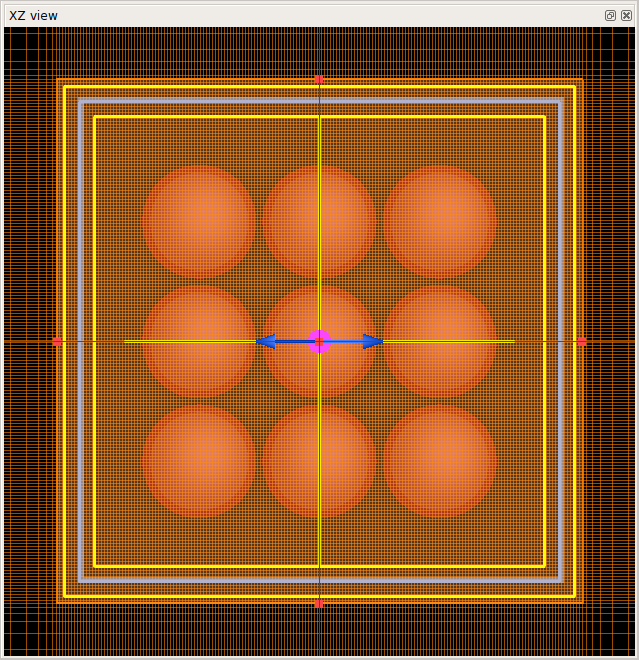
\includegraphics[width=0.95\textwidth]{fdtd-3x3}
  \end{minipage}
  \begin{minipage}[h]{0.49\textwidth} 
   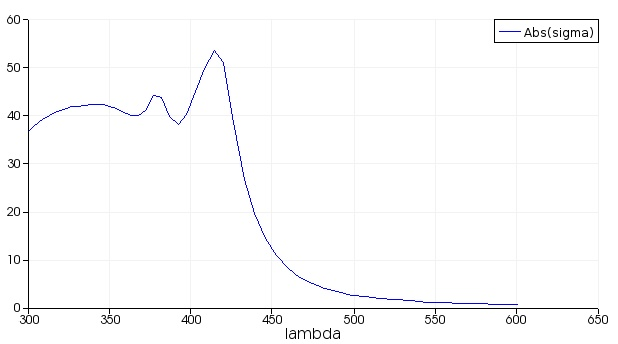
\includegraphics[width=0.95\textwidth]{fdtd-spectra-3x3}
  \end{minipage}
  \begin{minipage}[h]{0.49\textwidth}    \begin{flushleft}     c)    \end{flushleft}
  \end{minipage}
  \begin{minipage}[h]{0.49\textwidth}    \begin{flushleft}     d)   \end{flushleft}
  \end{minipage}
  \begin{minipage}[h]{0.49\textwidth} 
    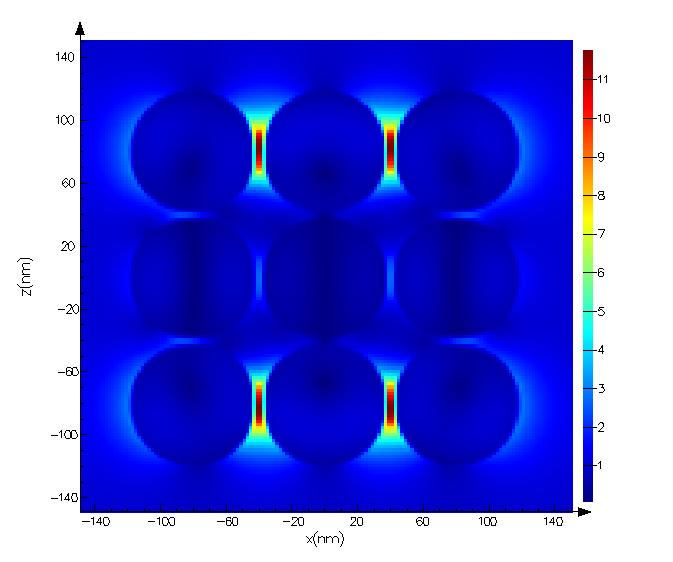
\includegraphics[width=0.95\textwidth]{fdtd-field-408nm}
  \end{minipage}
  \begin{minipage}[h]{0.49\textwidth} 
    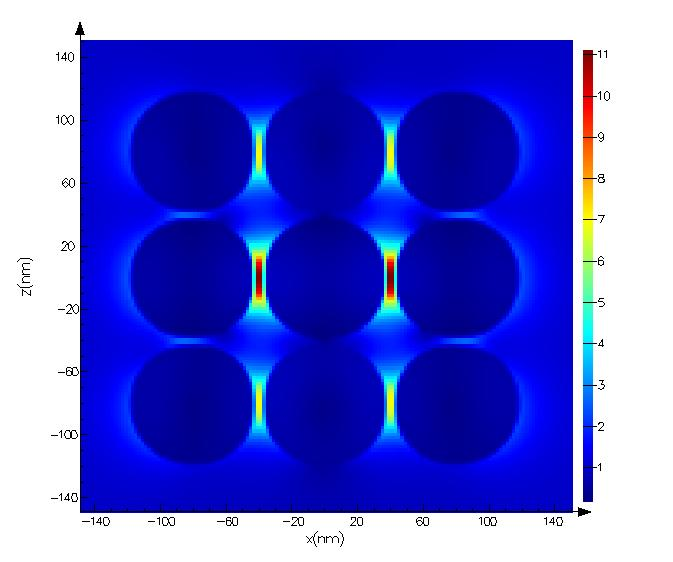
\includegraphics[width=0.95\textwidth]{fdtd-field-452nm}
  \end{minipage}
  \begin{minipage}[h]{0.49\textwidth}    \begin{flushleft}     e)    \end{flushleft}
  \end{minipage}
  \begin{minipage}[h]{0.49\textwidth}    \begin{flushleft}     -   \end{flushleft}
  \end{minipage}
  \begin{minipage}[h]{0.49\textwidth} 
    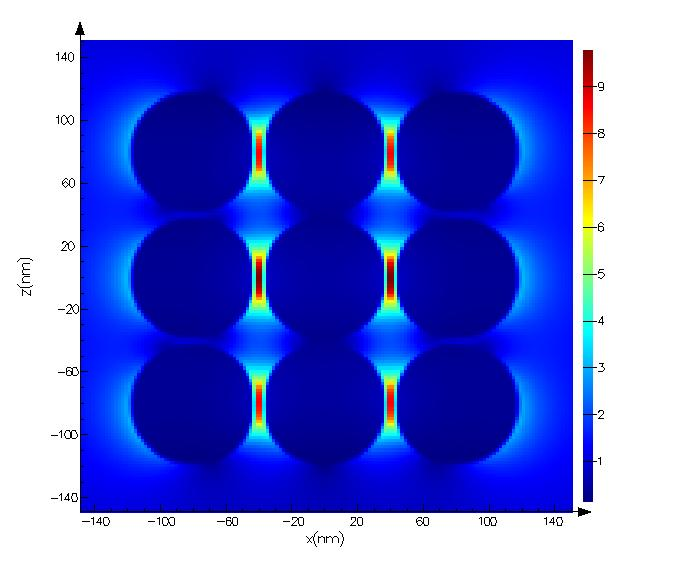
\includegraphics[width=0.95\textwidth]{fdtd-field-600nm}
  \end{minipage}
  %% \begin{minipage}[h]{0.49\textwidth} 
  %%   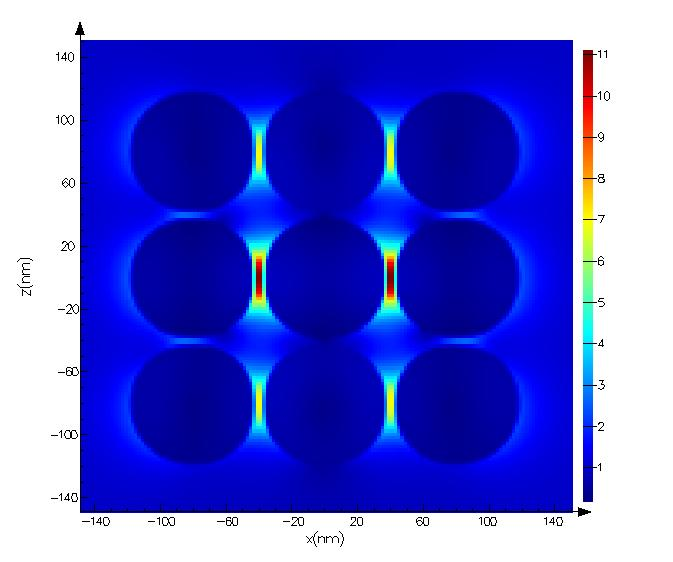
\includegraphics[width=0.95\textwidth]{fdtd-field-452nm}
  %% \end{minipage}
  
    \caption{ FDTD simulation of 3x3 grid of spheres optimized for
      absorption at 525~nm(a) Fullwave simulation prepared in
      Lumerical FDTD. (b) Cross-section absorption spectra (c,d,e)
      Field distribution at 408, 452, and 600nm of incident light.\label{fig:fdtd-3x3}}%
\end{figure}

Materials Letters 158, 262265 (2015) titled ``Dielectric shell
modulated plasmonic crystal for novel light absorption meta-surface''
provide another type of plasmonic coupling. In contrast to most other
works with hot spots located between the particles it this paper field
distributions presented in Fig 2 (b-d) is mostly localized inside the
particles and in Fig 2 (e) it is about the same order inside and
between the particles. It looks to be quite reasonable as far as
relatively small metallic core (d=25~nm) is covered with thick
dielectric shell (d=65~nm). This way due to relatively small coupling
between the particles we should expect to find this resonances in a
stand-alone particle, which was easy to reproduce. The result of Mie
calcultion for gold sphere (material data is from P. B. Johnson and
R. W. Christy. Optical Constants of the Noble Metals, Phys. Rev. B 6,
4370-4379 (1972)) of diameter d=25~nm covered with lossless and
dispersionless dielectric with refractive indes n=2.5 and d=65~nm in
Fig.~\ref{fig:Au-core-shell}. However, there was the only one electric
dipole resonance at 637~nm, futhermore, 3D FDTD simulation of such a
particle with a gold substrate (as is was used in the paper) and
periodic boundary condition for a HCP array lead to appearance of a
peak at 666~nm (for polarization oriented to far neighbor) in
Fig~\ref{fig:Au-core-shell}(c)  in contrast
with the simulation presented in Fig. 1(b) of the paper with several
resonances in range 700-1100~nm.  We do not
have a good explanation for such a disagreement.
\begin{figure}
  \includegraphics[width=0.95\textwidth]{Au-core-shell}\\
  c)\\
   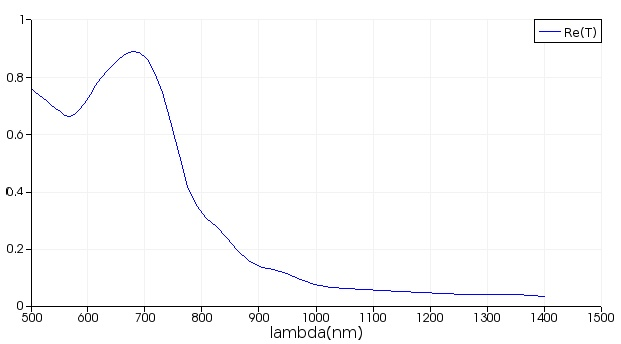
\includegraphics[width=0.95\textwidth]{fdtd-hcp}
  \caption{Mie simulation for core-shell particle with gold core (a)
    Mie absorption coefficients (b) Mie efficency for scattering,
    absorbtion, extinction and backscattering.(c)\label{fig:Au-core-shell}}
\end{figure}


This way it looks that using particle array adds a whole banch of new
physical features which deserve a separate investigation. No changes
to the manuscript were done.


%% We totally agree with the reviewer's statement. It seems that our
%% manuscript was not clear enough at this point. ...  However, as we
%% compare final optimization results we conclude that .... To make it
%% clearer we rewrite this part of the manuscript as follows:

%% \begin{tabular}[!H]{p{0.9\textwidth}}
%% `` Some text''
%% \end{tabular}

%% It should be mentioned that .... No changes to the
%% manuscript were made.

\vspace{10pt}

\newpage
\begin{minipage}{1.0\linewidth}
  \textbf{Reviewer \#2 comments}\\
  \begin{tabular}[!H]{l|p{0.9\textwidth}}
    \quad & 1.  As we can find from the manuscript, the highest
    absorption efficiency is achieved for a Si/Ag core-shell
    structure, which is not located in the super absorbing
    regime. Moreover, the authors also claimed that from practical
    aspect, the core-shell structure (not in the super absorbing
    regime) could be easier and cheaper to fabricate than three
    layered structure (in the super absorbing regime). Therefore, the
    authors should clearly clarify what are the advantages or
    significances of the super absorption nanoparticles? 
\end{tabular}
\end{minipage}

We added a sentence to the end of first paragraph of page 3 right
column after ``From a practical point of view, it is
quite important that the maximum can be reached in a bi-layer
structure, instead of a triple-layer, since it should be easier and
cheaper to fabricate.''

New sentencs: ``At the same time the best absorption efficency for
large particles (with $R>60$~nm for provided materials and layers
order) was achieved with superabsorption designs, which can be
relevant for the case of layer thickness fine control is not
available.''


%% Для маленьких толщин лучше простой диполь, если есть ограничения на
%% минимальный размер частицы - лучше суперпоглотитель. Или, например,
%% если важно ещё и абсолютное поглощение от одиночной частицы - большая
%% частица поглощает больше, для неё оптимальнее работа в супер- режиме. 


%% There are several points to be treated carefully when discussing...
%%  However, to claim this concept to be a general one ...  more simulations
%% should be performed.

\begin{tabular}[!H]{l|p{0.9\textwidth}}
  \quad &  2.      In Fig. 2, we noticed a discontinuity at ~80
  nm. The authors explain it as the design supporting electric dipole
  and magnetic quadrupole has larger ACS. However, this explanation is
  not clearly to me since it is lacking physics behind this
  phenomenon. The authors should clarify why the magnetic quadrupole
  only plays a significant role in this small wavelength range. 
\end{tabular}

The sort answer it that it was not possible to fit magnetic quadroupole to the particle of
smaller size, however, it is hard to keep it been efficient for larger
sizes. However, the contribution of the electric diple is also
very important.

To present this idea in more details we run an optimization with
changed fitness function - we requested to maximize the impact of
electric dipole to the absorption efficiency.

\begin{figure}
  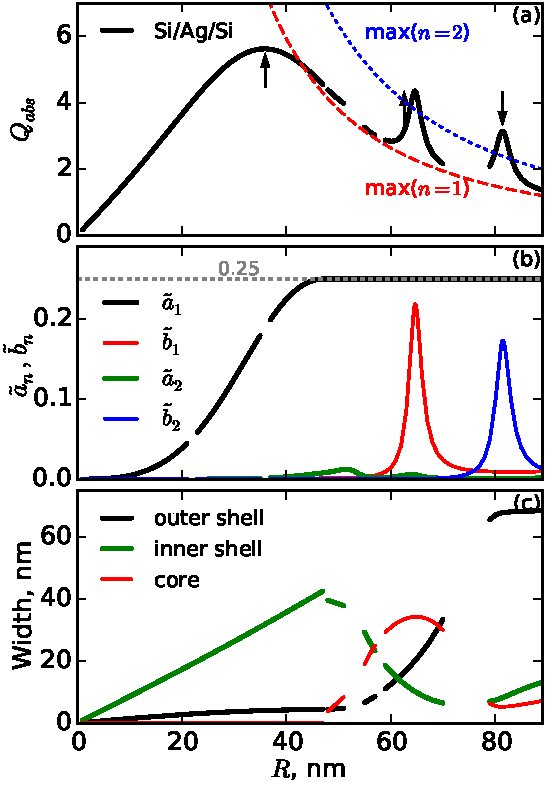
\includegraphics[width=0.35\textwidth]{overview-Qabs-a1}
  d)
   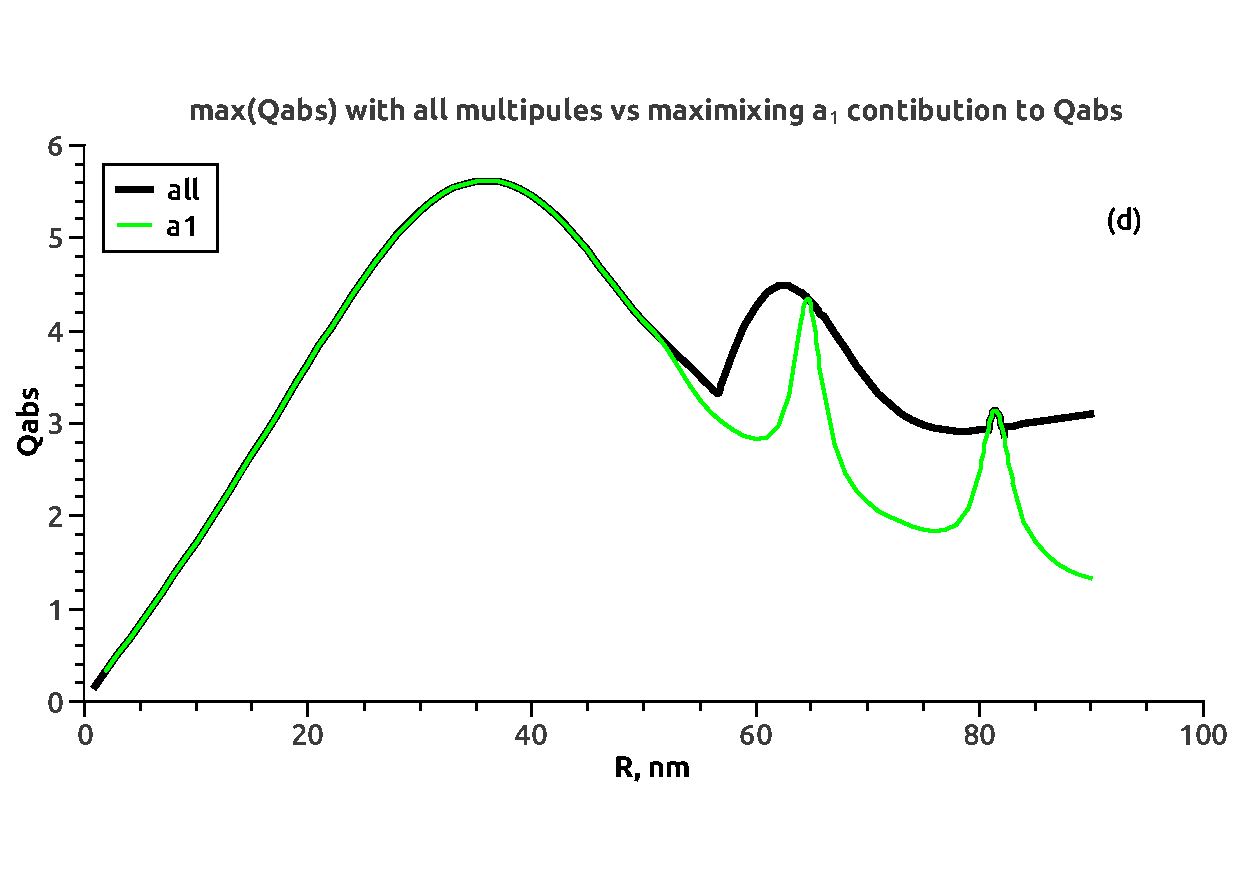
\includegraphics[width=0.55\textwidth]{overview-Qabs-all-a1}
  \caption{Mie simulation for core-shell particle with gold core (a)
    Mie absorption coefficients (b) Mie efficency for scattering,
    absorbtion, extinction and backscattering.(c)\label{fig:Au-core-shell}}
\end{figure}


\begin{tabular}[!H]{l|p{0.9\textwidth}}
\quad & 3.      In Fig. 3 (c), the authors observed a flat top of
electric dipole resonance. They attributed this flat resonance to the
excited several electric dipole resonances with close resonance
frequencies. Nevertheless, as we can see in Fig. 3 (d), even without
considering the resonances located in outer and inner shell, the
resonance inside the core is much broader than the other two
cases. The authors should explain this broadened resonance clearly. 
\end{tabular}

%% Да, он прав, основной вклад от ядра, остальные делают верхушку
%% плоской. Фишка в том что резонанс плоский, а не широкий.

\begin{tabular}[!H]{l|p{0.9\textwidth}}
\quad & 4.      Some sentences are not clear to me. For instance,
“there is a strong conterplay between the increased absorption for
larger particles vs size for smaller particles”. 
In summary, I do not think the manuscript is acceptable at its current
stage. 
\end{tabular}%
%% Илья
\\
\vspace{10pt}
\\
Sincerely Yours,\\
On behalf of the authors,\\
Konstantin Ladutenko
\end{document}
